% !TEX program = xelatex
%Wzór dokumentu
%tu zmień marginesy i rozmiar czcionki
\documentclass[a4paper,12pt]{article}
\usepackage{inputenc}[utf8]
\usepackage[margin=2.8cm]{geometry}
\usepackage[polish]{babel}

%Lepiej tego nie zmieniaj, jak co to dodawaj pakiety
\usepackage{titlesec}
\usepackage{titling}
\usepackage{fancyhdr}
\usepackage{mdframed}
\usepackage{graphicx}
\usepackage{amsmath}
\usepackage{amsfonts}
\usepackage{multicol}
\usepackage{listings}
\usepackage{caption}
\usepackage{float}
\usepackage{pdfpages}
\usepackage{tikz}
	\usetikzlibrary{arrows}



%inny wygląd
%\usepackage{tgbonum}


\usepackage{hyperref}
\hypersetup{
    colorlinks=true,
    linkcolor=blue,
    filecolor=magenta,      
    urlcolor=cyan,
}

\urlstyle{same}
%Zmienne, zmień je!
\graphicspath{ {./ilustracje/} }
\title{Tworzenie i uruchamianie prostych kontenerów w środowisku  docker-compose}
\author{Grzegorz Koperwas}
\date{\today}

%lokalizacja polska (odkomentuj jak piszesz po polsku)

\usepackage{polski}
\usepackage[polish]{babel} 
\usepackage{indentfirst}
\usepackage{icomma} 

\brokenpenalty=1000
\clubpenalty=1000
\widowpenalty=1000    

%nie odkometowuj wszystkiego, użyj mózgu
%\renewcommand\thechapter{\arabic{chapter}.}
\renewcommand\thesection{\arabic{section}.}
\renewcommand\thesubsection{\arabic{section}.\arabic{subsection}.}
\renewcommand\thesubsubsection{\arabic{subsubsection}.}

%Makra

\newcommand{\obrazek}[2]{
\begin{figure}[h]]
    \centering
    \includegraphics[scale=#1]{#2}
\end{figure}
}     

\newcommand{\stopnie}{\ensuremath{^{\circ}}}

\newcommand{\twierdzonko}[1]{
    \begin{center}
    \begin{mdframed}
    #1
    \end{mdframed}          
    \end{center}
} 

\newcommand{\dwanajeden}[2]{
\ensuremath \left( \begin{array}{c}
    #1\\
    #2
\end{array} \right)
}  

%Stopka i head (sekcja której nie powinno się zmieniać)
\pagestyle{fancy}
\fancyhead{}
\fancyfoot{}

%Zmieniaj od tego miejsca
\rfoot{\thepage}
\lfoot{}
\lhead{}
\rhead{Ostatnia edycja: \today}
\renewcommand{\headrulewidth}{1pt}
\renewcommand{\footrulewidth}{1pt}



\begin{document}
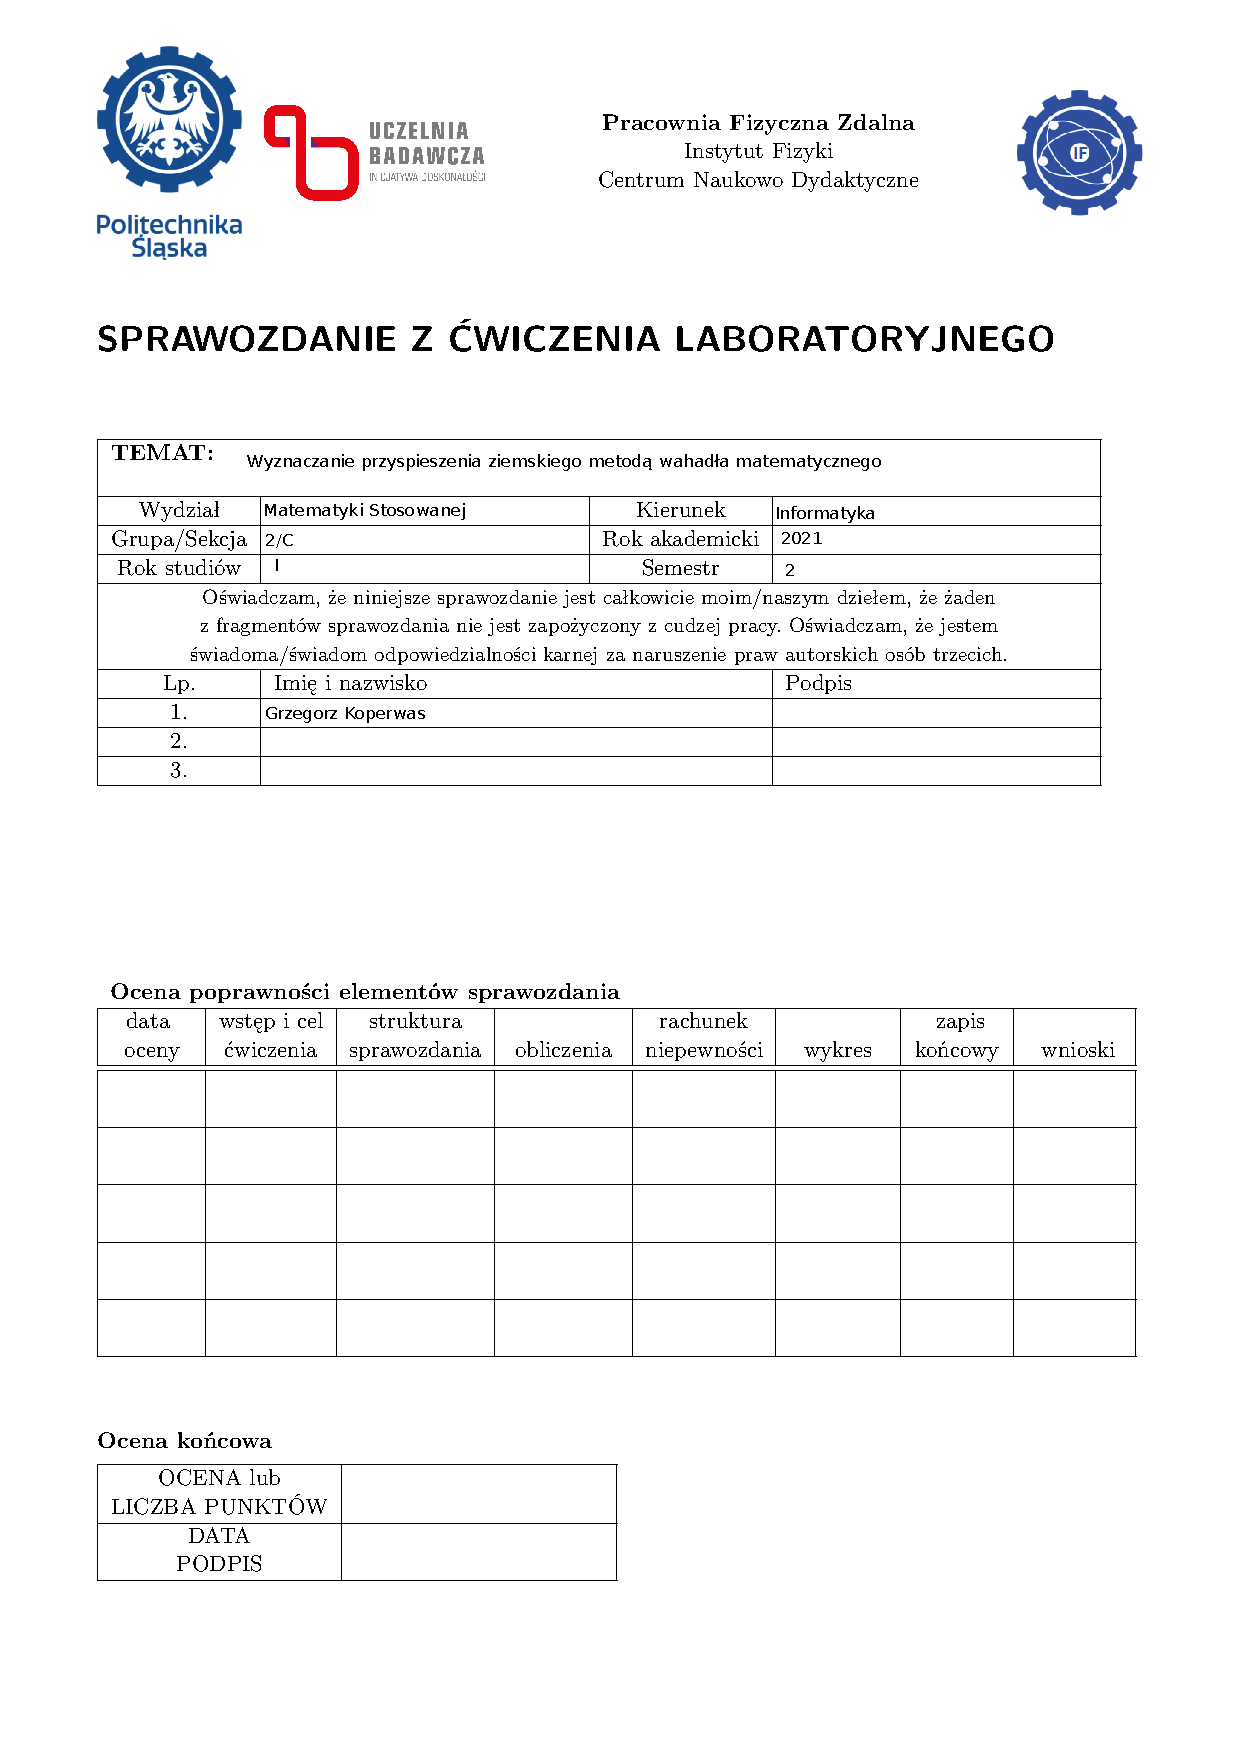
\includepdf[pages=-]{PFZ-StrTytulowaWyp.pdf}

\section{Wstęp teoretyczny}

Celem doświadczenia jest wyznaczenie przyspieszenia grawitacyjnego $g$ poprzez pomiar czasu w jakim wahadło wykona daną ilość cykli w zależności od jego długości.

\begin{figure}[h]
		\begin{tikzpicture}[scale = .7]
			\draw [dashed] (0, 0) -- (0, -6);
			\draw [dashed] (0, 0) -- (3, -5) [fill = black] circle [radius = .15];
			\node at (1.5, -2.25) [above] {$l$};
			\draw [->, thick] (3, -5) -- (3, -7) node [below]{$\vec{Q}$};
			\draw [->, thick] (3, -5) -- (2.25, -3.75) node [above]{$\vec{N}$};
			\draw [rotate = 270] (1, 0) arc (0:30:1);
			\node at (.18, -.6) {$\alpha$};
			\draw [rotate = 270, scale = 5.83, dashed] (1, 0) arc (0:30:1);
			\draw ( 0, -5 ) -- ( 3, -5 );
			\node at (1.5, -5) [above] {$x$};
			\node at (1.5, -5.7) [above] {$s$};
		\end{tikzpicture}
		\centering
		\footnotesize{
			\begin{itemize}
				\item $Q$ - ciężar
				\item $N$ - naciąg
			\end{itemize}
		}
		\caption{Wahadło w stanie największego wychylenia}
		\label{rys:wahadło}
\end{figure}

Wahadło matematyczne składa się z ciężarka, (Na rysunkach \ref{rys:wahadło} oraz \ref{rys:wahadło_siły} oznaczony jest jako kropka), który porusza się po łuku (jego długość to $s$).

Na potrzeby naszego eksperymentu rozważamy małe drgania wahadła, gdzie $\alpha < 7\stopnie$, zatem możemy założyć\cite{teoria:pw}:
\begin{equation}
	\sin \alpha \approx \alpha
\end{equation}\label{eq:smallAngle}

\begin{figure}[h]
		\begin{tikzpicture}[scale = .7]
				\draw [fill = black] (0,0) circle [radius = 0.15];
				\draw [->, thick] (0,0) -- (0, -4) node [below]{$\vec{Q}$};
				\draw [->, thick, rotate = 30] (0,0) -- (0, -3.46) node [below]{$\vec{Q_1}$};
				\draw [->, thick, rotate = -60, scale= 0.5] (0,0) -- (0, -4) node [below]{$\vec{Q_2}$};
				\draw [->, thick, rotate = 210] (0,0) -- (0, -3.46) node [above]{$\vec{N}$};
				\draw [rotate = 270, scale = 1.5](1,0) arc (0:30:1);
				\node at (.27,-.9){$\alpha$};
				\draw [dashed, thin, rotate = -60](0,0) arc (0:-30:12);
		\end{tikzpicture}
		\centering
		\footnotesize{
			\begin{itemize}
				\item $Q$ - ciężar
				\item $N$ - naciąg
			\end{itemize}
		}
		\caption{Rozkład sił na wahadle}
		\label{rys:wahadło_siły}
\end{figure}

Na rysunku \ref{rys:wahadło_siły} widzimy iż siła $\vec{Q_1}$ jest równoważona przez siłę $\vec{N}$, zatem siła $\vec{Q_2}$ jest siłą wypadkową. 

\begin{align*}
	\vec{Q} &= m\vec{g} \\
	\left|Q_2 \right| &= mg\sin{\alpha} = mg\frac{x}{l}, \quad \text{Z (\ref{eq:smallAngle})} \\
	\left| Q_2  \right| &\approx mg \frac{s}{l}
\end{align*}

Siła $\vec{Q_2}$ jest zwrócona do środka, zatem:

\begin{equation*}
	Q_2 = - \frac{mg}{l}s
\end{equation*}

Siła ta jest zależna od wychylenia wahadła, zatem jest ona siłą sprężystą\cite{teoria:force} w formie $F = -kx$, gdzie:
\[k = \frac{mg}{l}, \quad x = s\]

Zatem układ wykonuje ruchy harmoniczne, gdzie okres drgań $T$ jest dany wzorem:

\begin{align*}
	T &= 2 \pi \sqrt{\frac{m}{k}} = 2 \pi \sqrt{\frac{m}{\frac{mg}{l}}} = \\
	&= 2 \pi \sqrt{\frac{l}{g}}
\end{align*}

Następnie wyliczamy z wzoru $g$:

\begin{align*}
	T^2 &= 4 \pi^2 \cdot \frac{l}{g} \\
	g &= \frac{4 l \pi^2 }{T^2}
\end{align*}

Na potrzeby sprawozdania obliczymy $g$ jako nachylenie wykresu liniowego:

\begin{align*}
	T^2 &= 4 \pi^2 \cdot \frac{l}{g} \\
	T^2\left(l\right) &= \frac{4 \pi^2}{g} \cdot l
\end{align*}

Gdzie nachylenie wykresu $T^2 \left(l\right)$ to $\frac{4 \pi^2}{g}$.

\bibliographystyle{alpha}
\bibliography{Sprawozdanie}
\end{document}
